\subsection[Operator product expansion for \btokpipimumu and \btophikmumu]
{Operator product expansion for $\boldsymbol{\btokpipimumu}$ and $\boldsymbol{\btophikmumu}$}

The effective Hamiltonian for the \fcnc $\decay{b}{s\ell^+\ell^-}$ is given by:
\begin{equation}
  \Ham{eff} = -4\frac{G_F}{\sqrt{2}}\Vconj{ts}\V{tb}\frac{e^2}{16\pi^2}
  \sum_{i}\big[c_i(\mu)\mathcal{O}_i(\mu)+c_i(\mu)^\prime\mathcal{O}_i^\prime(\mu)\big]
\end{equation}
similar to \Eq{eq:th:lageff}, where the coefficients are known as Wilson coefficients, which
correspond to the Wilson operators $\mathcal{O}_{1-10}$.
The operators $\mathcal{O}_{1-6}$ are sensitive to long distance contributions such as \ccbar
loops.
Operators which are particularly sensitive to NP contributions in \decay{b}{s\mumu} transitions are
\begin{align}
  \Op{7\pz} &= \frac{m_b}{e}\big(\bar s \sigma_{\mu\nu}P_Rb\big)F^{\mu\nu}
  %$\bra{f}\Op}\ket{i}$.
  &\Op{7\pz}^\prime &= \frac{m_b}{e}\big(\bar s \sigma_{\mu\nu}P_Lb\big)F^{\mu\nu}
  \nonumber\\
  %\mathcal{O}_8 &= g\frac{m_b}{e^2}\big(\bar s \sigma_{\mu\nu}T^aP_Rb\big)G^{\mu\nu a}
  %&\mathcal{O}_8^\prime &= g\frac{m_b}{e^2}\big(\bar s \sigma_{\mu\nu}T^aP_Rb\big)G^{\mu\nu a}
  %\\
  \Op{9\pz} &= \big(\bar s\gamma_\mu P_Lb\big)\big(\bar\ell\gamma^\mu\ell\big)
  &\Op{9\pz}^\prime &= \big(\bar s\gamma_\mu P_Rb\big)\big(\bar\ell\gamma^\mu\ell\big)
  \nonumber\\
  \Op{10} &= \big(\bar s\gamma_\mu P_Lb\big)\big(\bar\ell\gamma^\mu\gamma_5\ell\big)
  &\Op{10}^\prime &= \big(\bar s\gamma_\mu P_Rb\big)\big(\bar\ell\gamma^\mu\gamma_5\ell\big)
  \phantom{\frac{1}{1}}
  %\\
  %\mathcal{O}_{S} &= \frac{m_b}{m_{B_s}}\big(\bar s\gamma_\mu P_Rb\big)\big(\bar\ell\ell\big)
  %\\
  %\mathcal{O}_{P} &= \frac{m_b}{m_{B_s}}\big(\bar s\gamma_\mu P_Rb\big)\big(\bar\ell\gamma_5\ell\big)
\end{align}
where $P_{L,R}$ are the left and right projection operators.
The operators \Op{7} and \Op{9} describe the emission of a photon or $Z$ from a penguin loop,
and \Op{10} corresponds to a box type diagram with \Wp; these are shown in \Fig{fig:hhh:loops}.
Primed operators are the suppressed helicity, whose contributions are vanishingly small in the SM.


\begin{figure}
  \begin{center}
    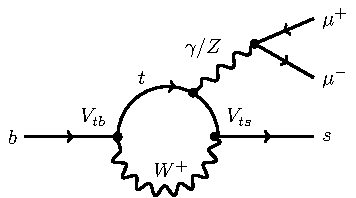
\includegraphics[scale=1]{feynman_btosmumu_penguin}
    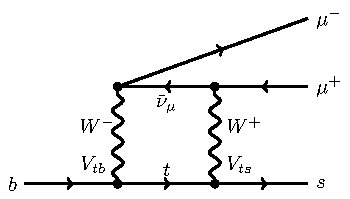
\includegraphics[scale=1]{feynman_btosmumu_box}
    \caption[Schematic Feynman diagrams for loop and box diagrams]
    {
      Schematic Feynman diagrams for the
      (left) penguin loop diagrams corresponding to the operators \Op{7} and \Op{9} depending on
      whether a $\gamma$ or $Z$ is emitted from the loop;
      (right) \Op{10} box diagram mediated by \Wp bosons.
    }
    \label{fig:hhh:loops}
  \end{center}
\end{figure}

As well as in loops, virtual particles can also contribute in some tree level diagrams.
The small value of $|\V{ub}|$ means that annihilation decays of \Bp mesons are heavily
suppressed in the SM.
%They are mediated by
%Tree level diagrams in the SM are typically high statistics modes, however annihilation type decays
%are heavily suppressed.
These rare modes are propagated by a \Wp in the SM; but this could be exchanged for any charged
boson, such as an $H^+$ from SUSY, this could alter the branching fraction or
introduce significant CPV.
%The decay \btodsphi is an annihilation decay of the \Bp.










